\subsubsection*{The dynamic-OOBN model}
\label{Section:DaimlerDynamic}

The above described static OOBN is able to detect a manoeuvre $0.6$ seconds before execution. As detailed in the DoW \cite{Fer14}, the goal is to extend the prediction horizon for manoeuvre recognition to at least 1-2 seconds (max.\ $4-5$ seconds ahead) before the actual lane marking crossing. Moreover, this early detection of the manoeuvre should not be at the expense of the prediction accuracy;  as specified on Daimler's DoW \cite{Fer14}, the area under the ROC curve (AUC) should be greater than 0.96 for 1 second and greater than 0.9 for 2 seconds.

Figure \ref{Figure:daimlerTPlot} shows an example of the current performance and limitations of the static-OOBN model. They correspond to two randomly selected sequences in which we keep track of the behaviour of two cars, the EGO and the OBJECT. In these figures we plot the evolution of different time-steps for lateral velocity and lateral offset to a lane marking in ongoing Object-CutOut and Object-CutIn manoeuvres (as sketched in Figure \ref{Figure:DaimlerManeuvers}). The vertical black bar indicates the moment in which the manoeuvre has been recognised by the static-OOBN. The manoeuvre is finished at the end of the series, which coincides with the actual moment of changed lane. The black curve corresponds to the lateral offset and lateral velocity of the EGO car, which is just following the lane (LF), and the green curve corresponds to the values of the Object car performing the Object-CutOut/Object-CutIn manoeuvres. As expected for lane follow (LF), the lateral velocity of the EGO fluctuates around zero  (i.e., EGO car is just driving inside its lane) and the lateral offset of the lane marking is almost constant all the time. However, when we look at the lane change behaviour of the OBJ car (green lines), we easily see a quite different behaviour. Firstly, we observe that the lateral velocity is much  higher indicating a lateral movement. Similarly, we also observe how the lateral offset steadily increases, what clearly indicates that the Object car is leaving its current lane in both manoeuvres. 

\begin{figure}
\begin{center}
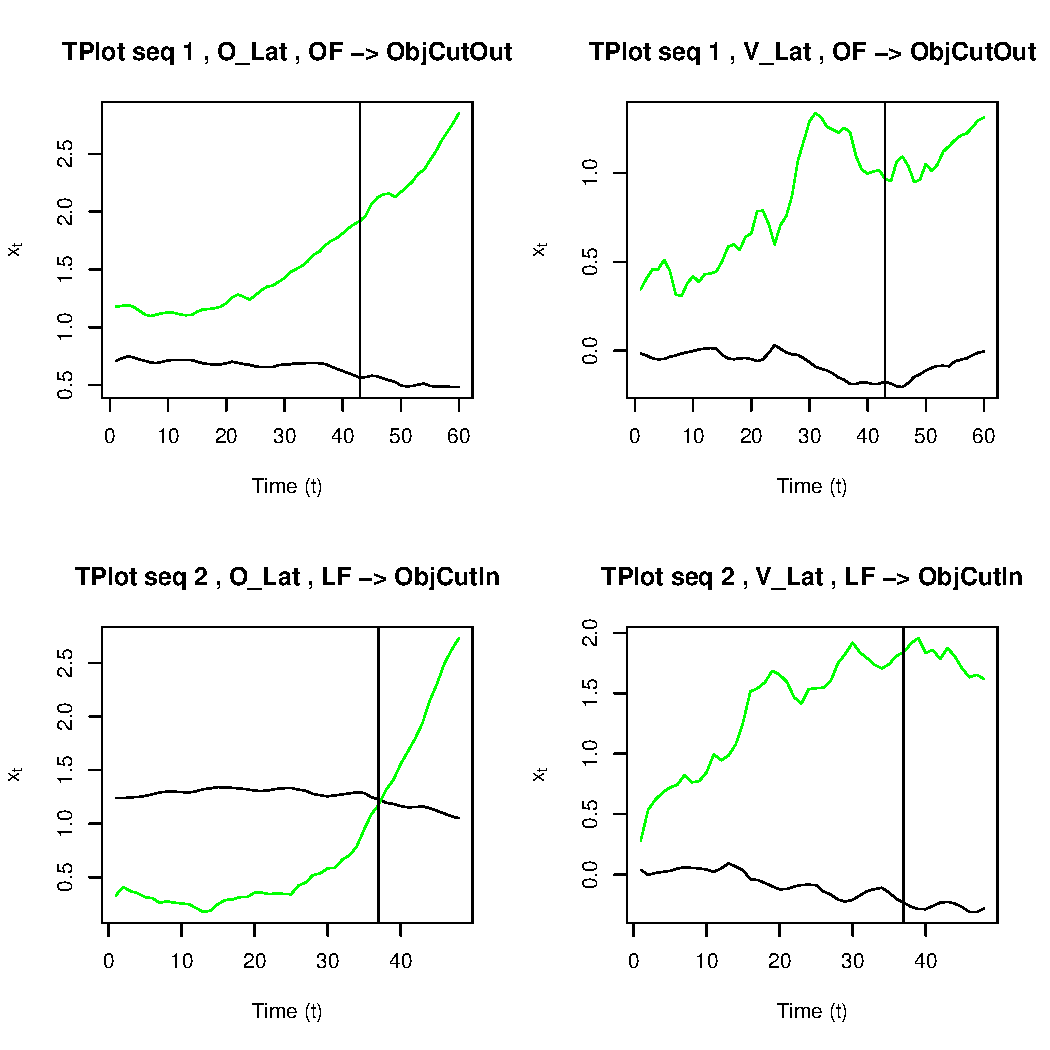
\includegraphics[scale=0.65]{./figures/DaimlerLE_EGO_L_LE_OBJ_R_OBJCut.pdf}
\caption{\label{Figure:daimlerTPlot}Daimler time plots of the lateral velocity and offsets for EGO (black line) and OBJECT (green line) in two randomly selected sequences of an ObjCutOut and an ObjCutIn. The x-axis corresponds to the different timesteps and the y-axis to the lateral offset on the left-hand side graphs and lateral velocity on the right-hand side graphs.}
\end{center}
\end{figure}


Although the manoeuvre is clearly identified before it completes in both cases, it is desired to predict it \textit{further} in advance. Looking at the evolution of lateral offset and velocity in Figure \ref{Figure:daimlerTPlot}, we could argue that the detection of the manoeuvre can be performed earlier (i.e. when the lateral offset and lateral velocity starts to increase more dramatically and consistently for \textit{several} timesteps). This is one of the basic pieces of evidence that motivates the development of the dynamic version of the static-OOBN model \cite{Weidl2014}.  Another piece of evidence appears when we look at the sample correlograms for lateral velocity and offset (that is, the correlation of the data with lagged values of themselfves) plotted in Figure \ref{Figure:daimlerCorrel}. There we can see a strong temporal dependency (the correlation coefficients are high) for the two variables when we consider a \textit{small} number of time steps between the temporal observations. Hence, the use of a dynamic model to make predictions about the evolution of the lateral velocity and lateral offset in a near future seems to be reasonable according to this analysis. And our main assumption is that the use of dynamic Bayesian network models (see Section \ref{Section:Preliminaries}) will allow us to build a more accurate and reliable system for manoeuvre recognition. 

\begin{figure}
  \centering
    \begin{tabular}{cc}
    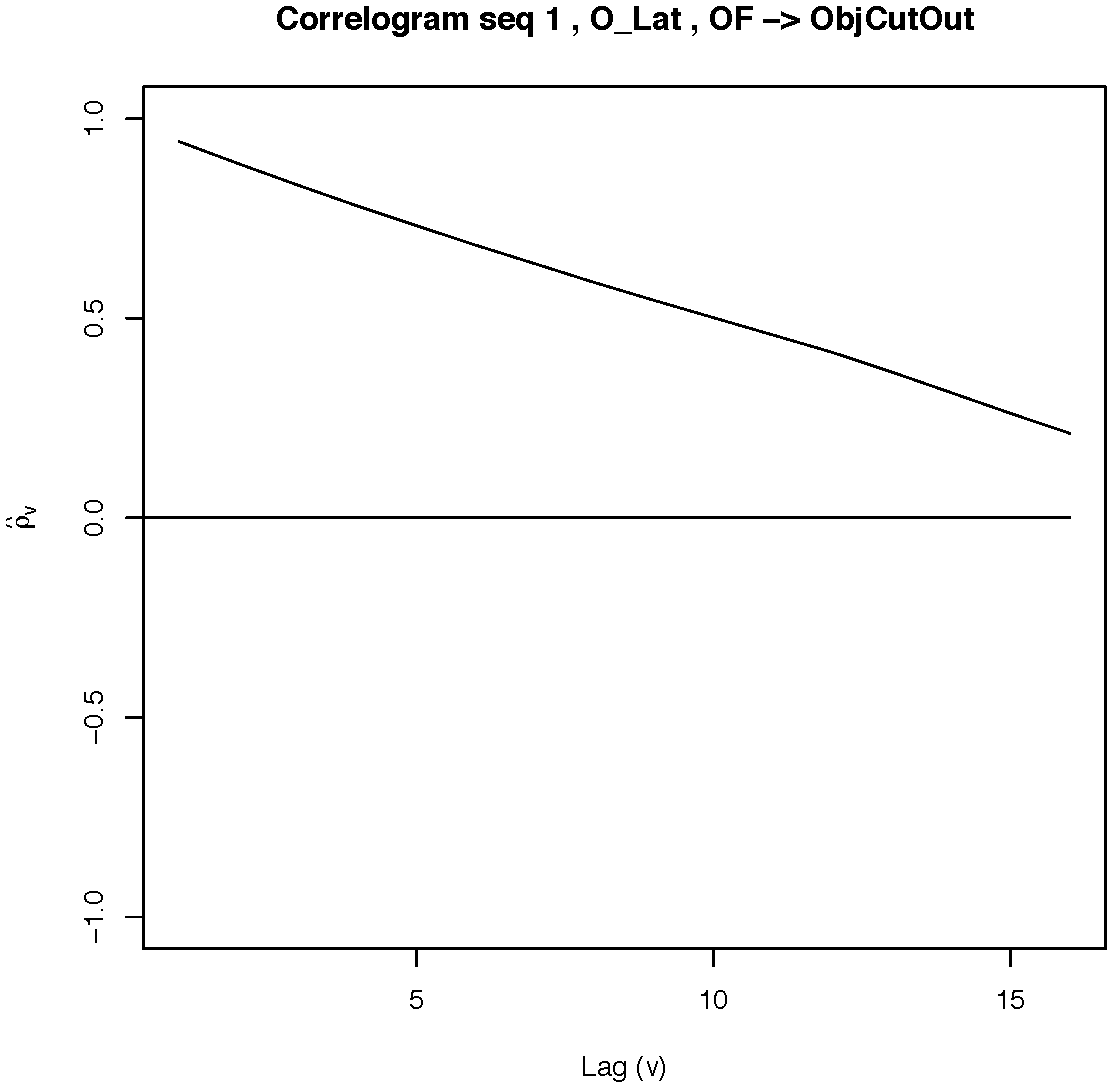
\includegraphics[width=60mm]{figures/DaimlerCorrOBJ_R15Offs.pdf}&
    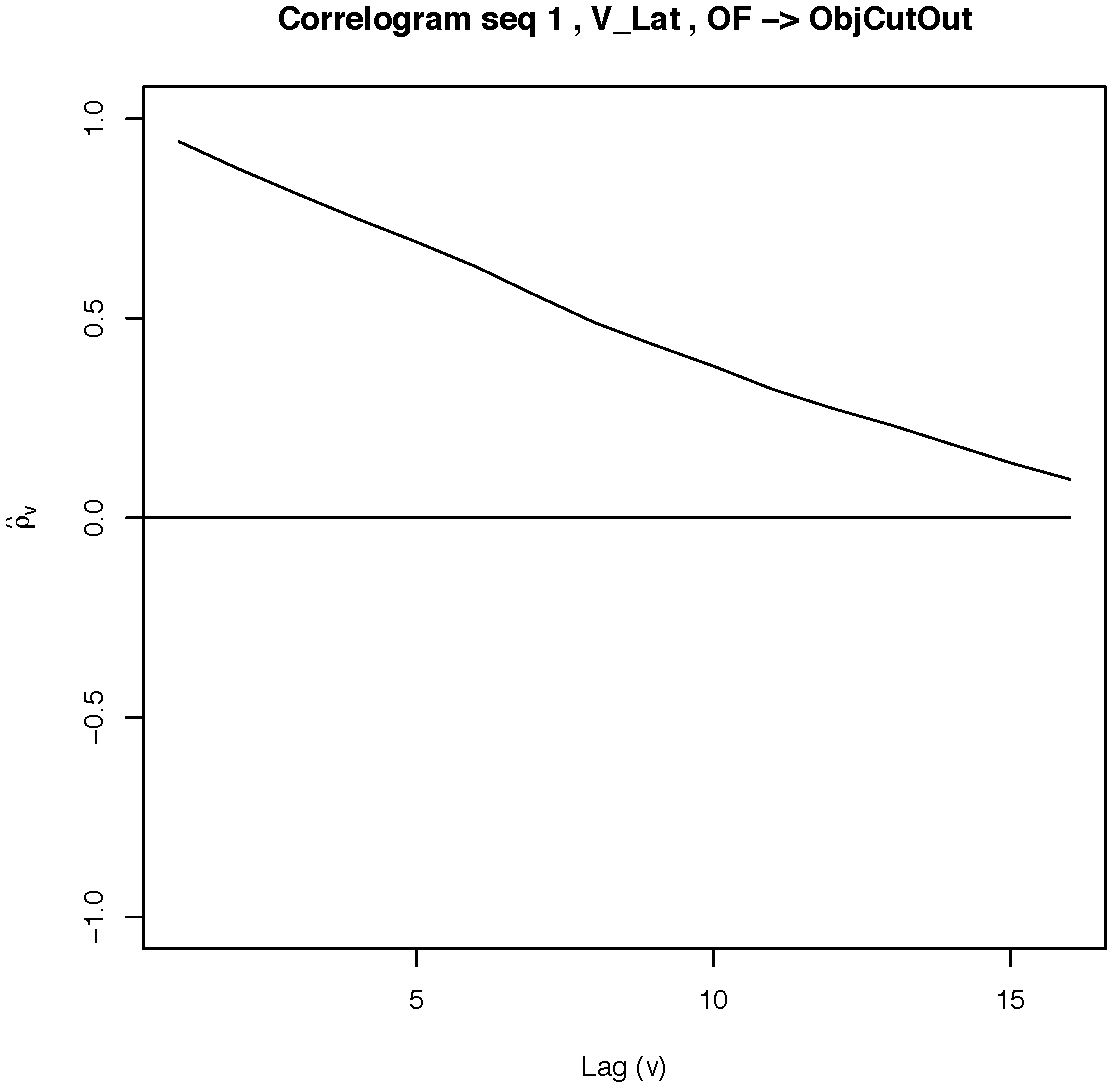
\includegraphics[width=60mm]{figures/DaimlerCorrOBJ_R15Vel.pdf}\\
  \end{tabular}
    \caption{\label{Figure:daimlerCorrel}Correlograms for Lateral velocity and offset. The x-axis represents the lag $v$ or time difference, and the y-axis the sample autocorrelation coefficient of lag $v$, $\hat{\rho_v}$, that is, the correlation between variables at time $t$ and at time $t+v$ (See Section \ref{Section:Preliminaries} for more details).}
\end{figure}

In any case, let us note however that the prediction horizon for manoeuvre recognition is going to be limited in order to avoid false positives (i.e. recognizing a lane change manoeuvre when the driver was just performing some random lateral movement).  In case of a false positive, such as an erroneously Object-CutIn for instance, the adaptive cruise control would react with an unnecessary break, so they ought to be avoided. It is then required to find a good balance between the rate of false positives and false negatives. 

\begin{figure}
\begin{center}
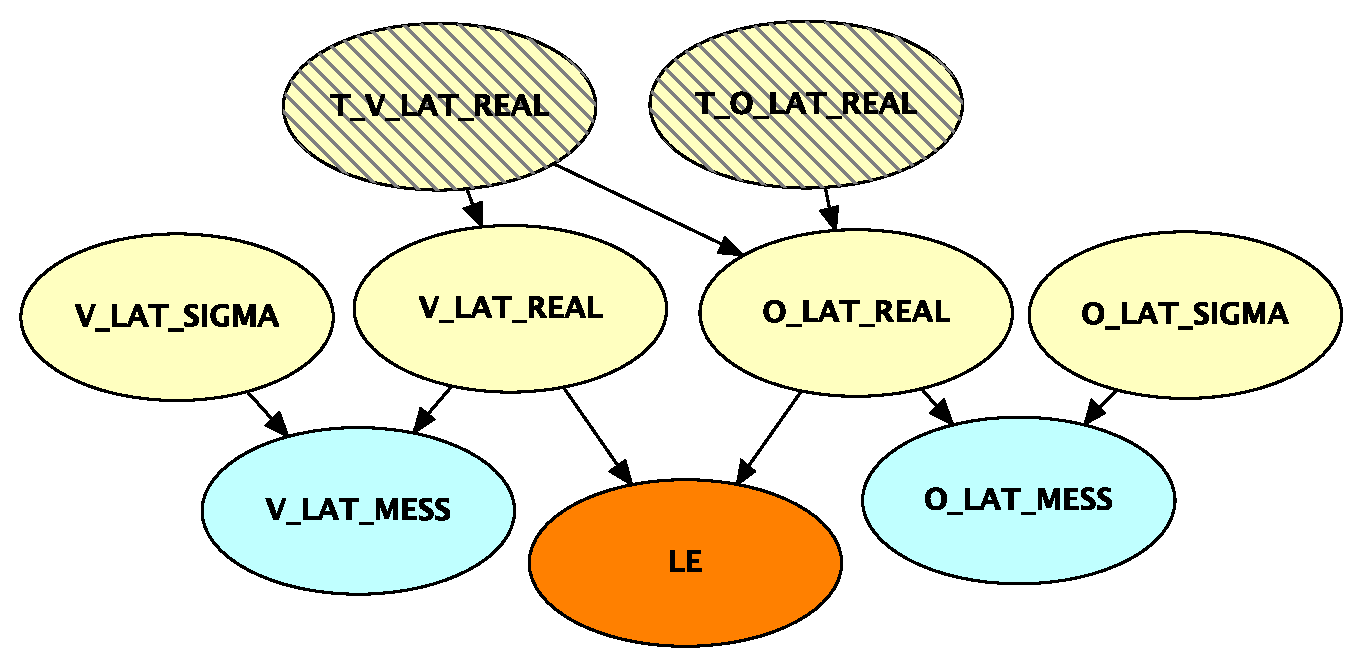
\includegraphics[scale=0.58]{./figures/DaimlerLEdyn}
\end{center}
\caption{\label{Figure:daimlerLEdyn}Daimler dynamic fragment for the LE hypothesis.}
\end{figure}

As explained in Section \ref{Section:Preliminaries}, the dynamic extension involves copies of the static OOBN for different number of time steps in the time window. Figure \ref{Figure:daimlerLEdyn} shows an example for the LE hypothesis, where the nodes for O\_LAT\_REAL and V\_LAT\_REAL are temporal clones defining the share belief state between consecutive time steps, and hence creating a first order Markov process. This model has been proposed in \cite{Weidl2014} by some of the AMIDST partners.  The first order assumption is a standard assumption in this kind of models and helps to simplify the posterior inference and learning process. Fortunately, if we build a partial-correlogram as the ones plotted in Figure \ref{Figure:daimlerPartialCorrel}, we can see that this assumption seems reasonable, because the influence of the lateral offset a time $t-1$ on the lateral offset at time $t+1$ given the lateral offset at time $t$ is close to null (i.e. the value at $v=2$ for the lag is close to null in Figure \ref{Figure:daimlerPartialCorrel}). And the same reasoning applies to the lateral velocity.

\begin{figure}
  \centering
    \begin{tabular}{cc}
        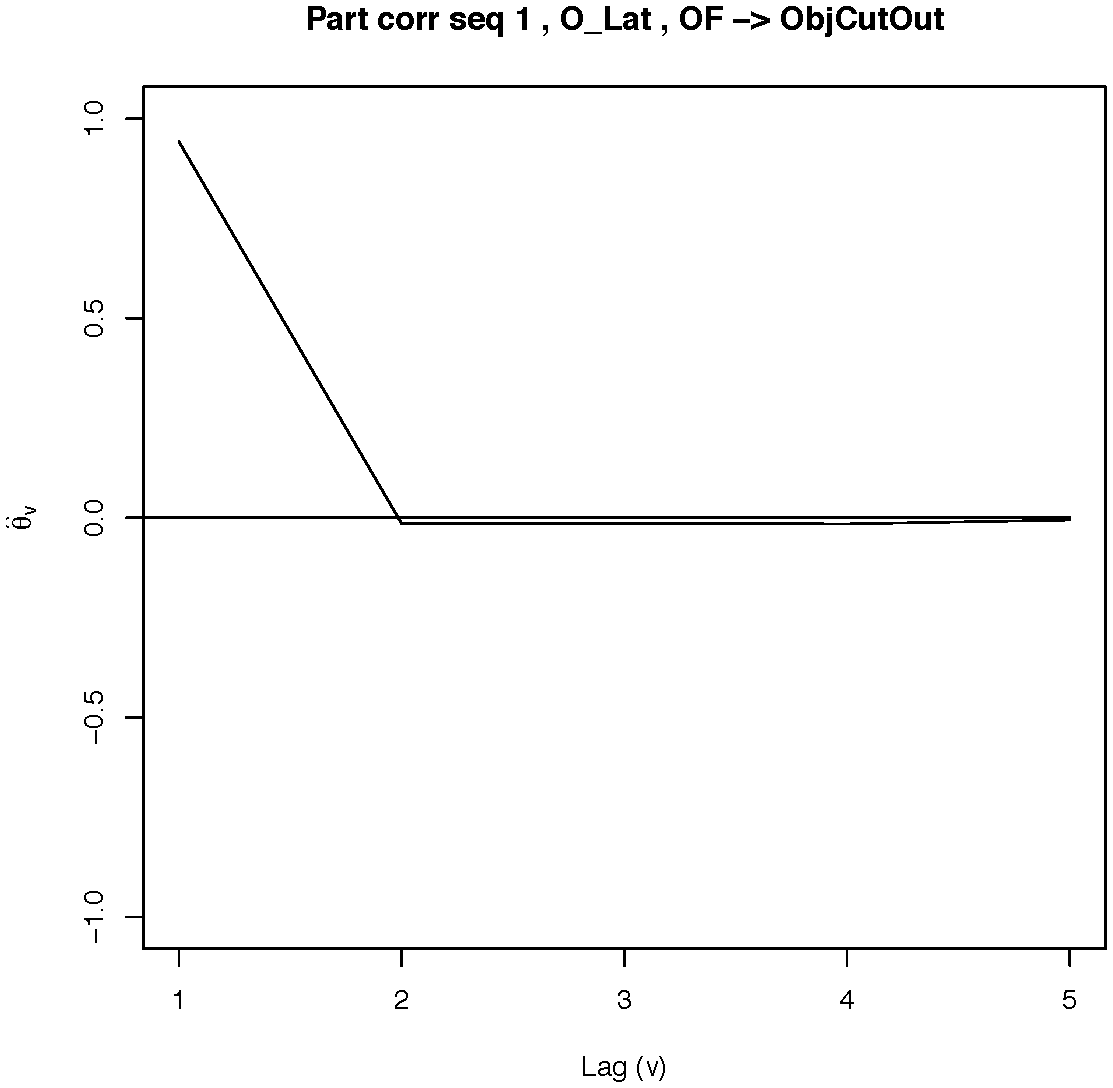
\includegraphics[width=60mm]{figures/DaimlerPcorrOBJ_R5Offs.pdf}&
    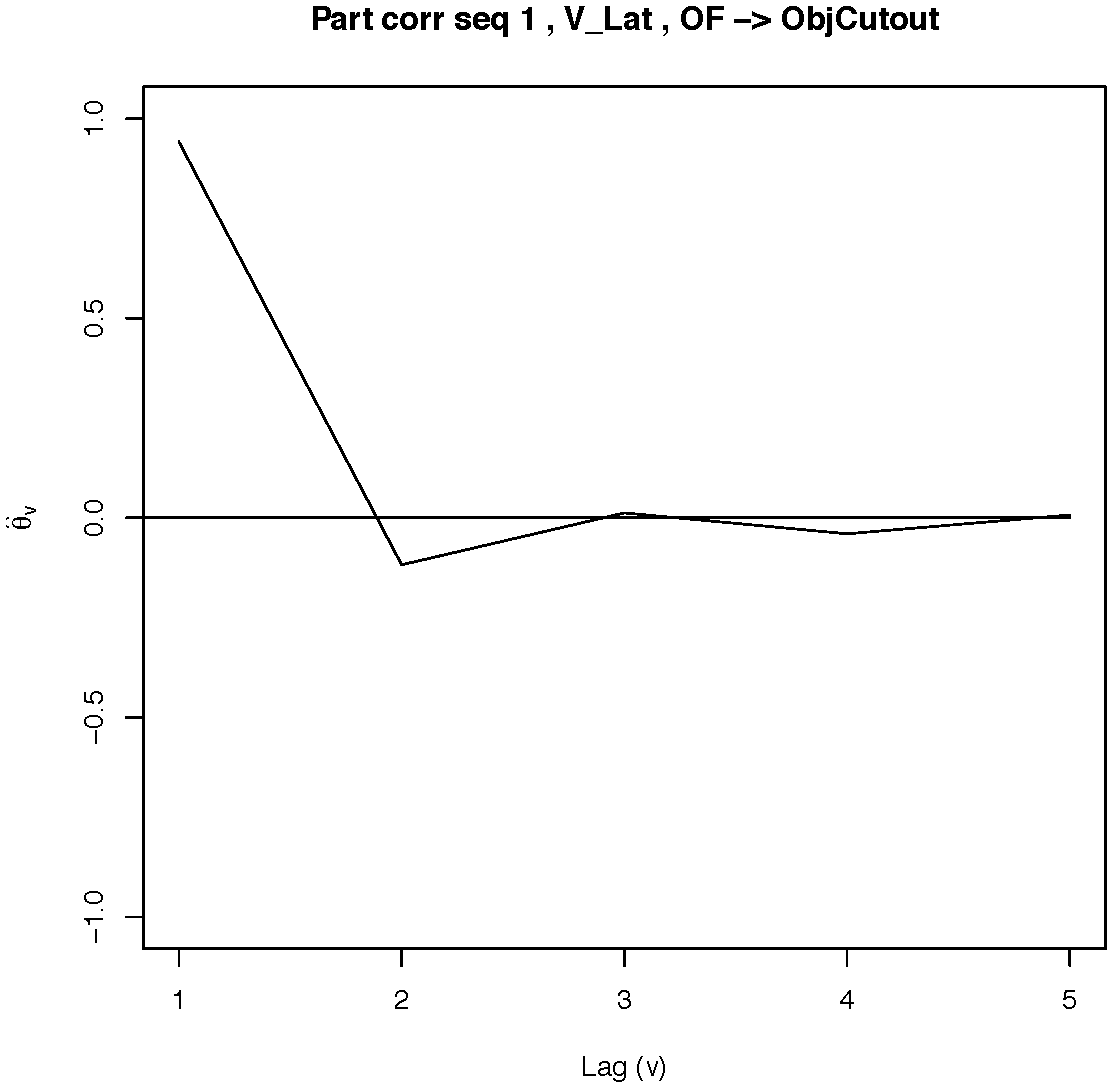
\includegraphics[width=60mm]{figures/DaimlerPcorrOBJ_R5Vel.pdf}\\
  \end{tabular}
    \caption{\label{Figure:daimlerPartialCorrel}Partial-correlograms for lateral velocity and offset. The x-axis represents the lag $v$ or time difference, and the y-axis the partial autocorrelation coefficient of lag $v$, $\ddot{\theta_v}$, that is, the correlation between variables at time $t$ and at time $t+v$ after having removed the common linear effect of the data in between. (See Section \ref{Section:Preliminaries} for more details).}
\end{figure}


As described in \cite{Weidl2014}, the proposed dynamic BN (DBN) aims to incorporate the trend of change for the real values, where their physical relations are represented as causal dependencies between the time steps $dt$. For instance, in Figure \ref{Figure:daimlerLEdyn} the transition function of O\_LAT\_REAL at time $t$, denoted by $O(t)$, is modeled as a Gaussian distribution. Its mean is affected by $O(t-1)$, and by V\_LAT\_REAL at time $t-1$, denoted by $V(t-1)$:

\begin{equation}
O(t) =O(t-1) +V(t-1)dt +\epsilon
\end{equation}

where $\epsilon$ denotes a white noise $\mathcal{N}(0,\sigma^2)$ which is assumed to be small. In order to corroborate the validity of this distributional assumption, we also analysed the hypothesis $O(t) - O(t-1) = \Delta O = V(t-1)dt +\epsilon$ on our data. Figure \ref{Figure:daimlerVvsOffs} shows the plot and contour plots for $V$ and $\Delta O$, which show that the assumption of linear relationship with Gaussian noise might not be very far from reality.

\begin{figure}
  \centering
  \setlength{\tabcolsep}{0.05pt}
  \renewcommand{\arraystretch}{0.02}
    \begin{tabular}{cc}
    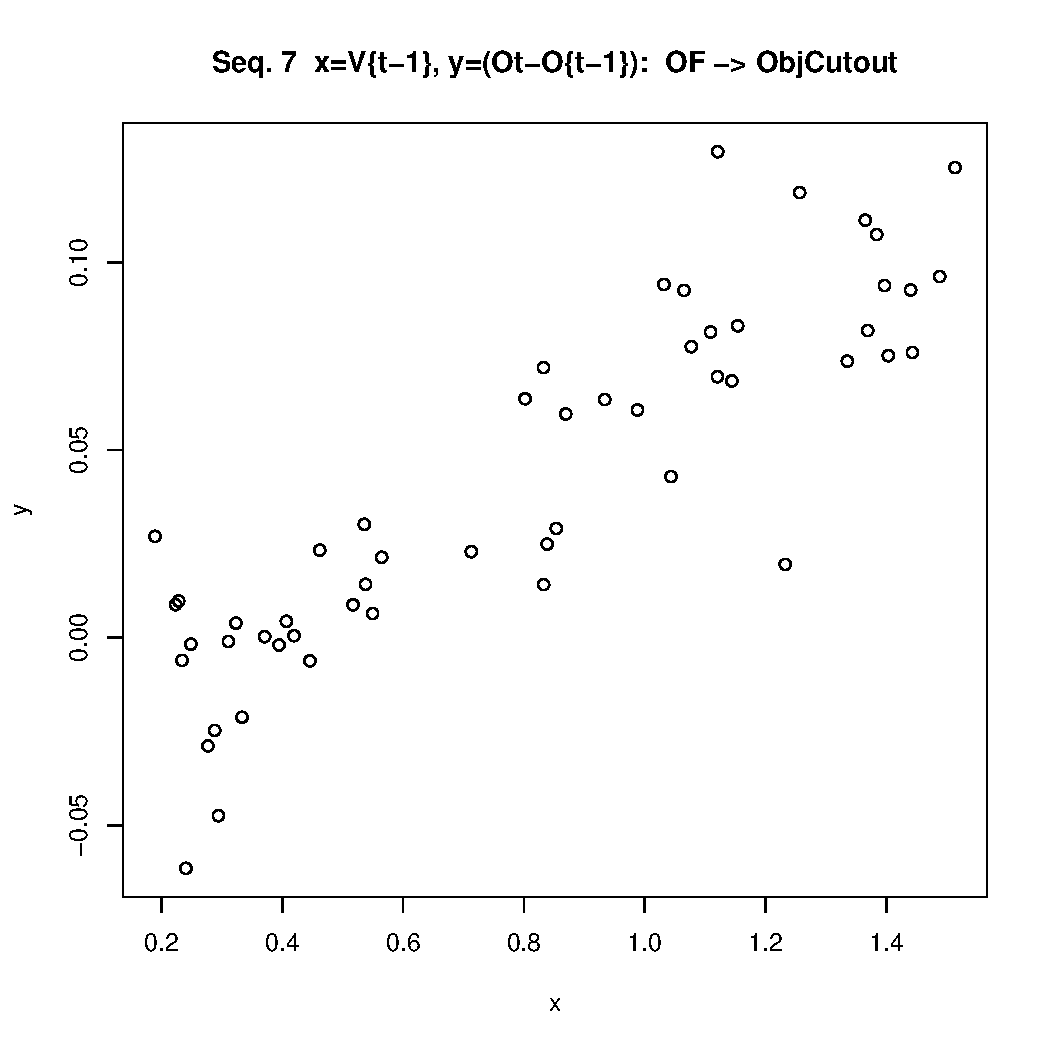
\includegraphics[width=60mm]{figures/DaimlerOBJplotSerie7.pdf}&
    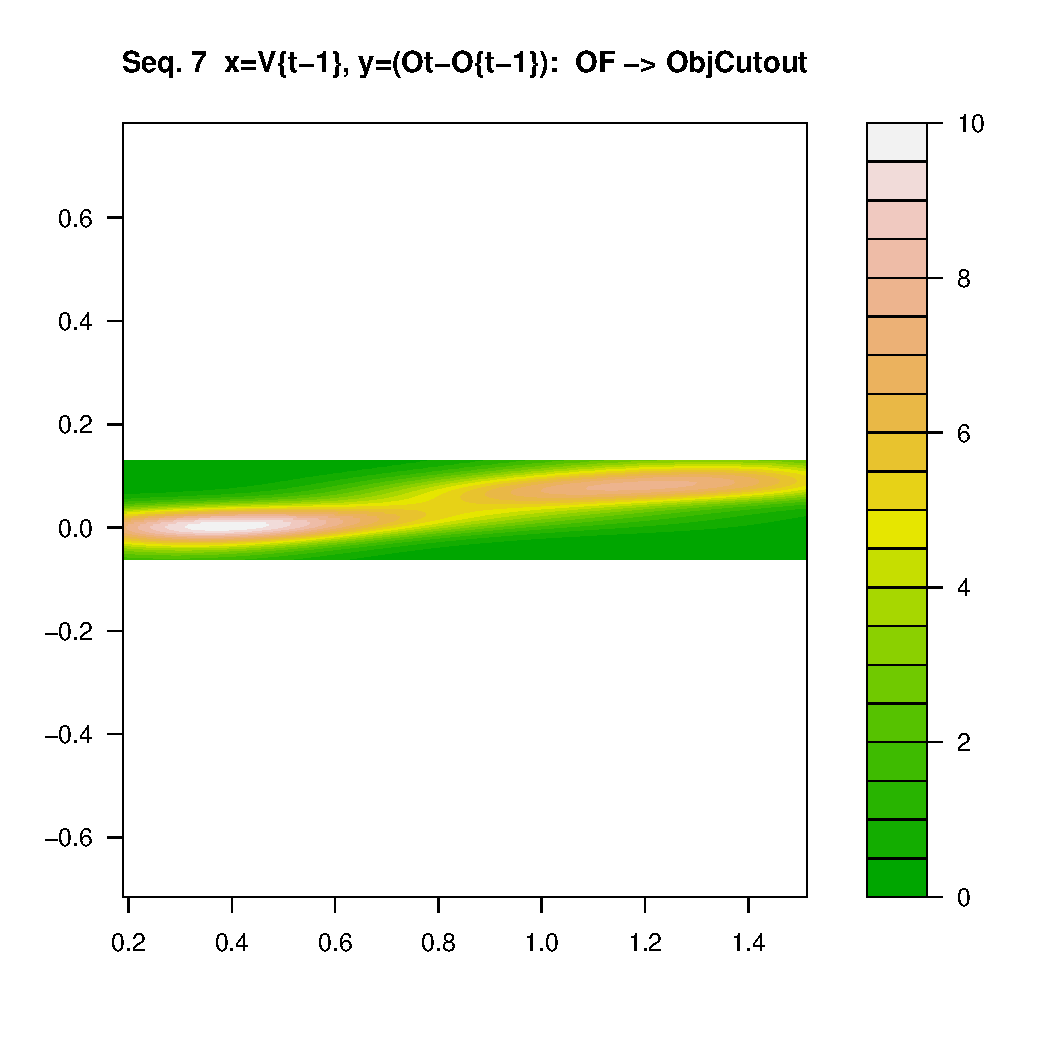
\includegraphics[width=60mm]{figures/DaimlerOBJcontourSerie7.pdf}\\
  \end{tabular}
      \caption{ \label{Figure:daimlerVvsOffs}Time plot for $V(t-1)$ vs $O(t) - O(t-1)$. Linear correlation can be observed.}
\end{figure}

%Additionally,  we believe that even earlier prediction of manoeuvre intentions could be achieved before any development of the trend for lateral evidence LE has been observed. A first indication of possible lane change intention can be observed through the relative dynamics between one vehicle (EGO or OBJECT) and the vehicles in front of it on the same lane. Once again, the goal is to further increase the prediction horizon for manoeuvre recognition (up to 5 seconds), and this approach will be further explored in future stages of the project. 

Finally, in Figure \ref{Figure:daimlerLEdynGeneric} we show a rough overview of the final structure of this dynamic Bayesian network\footnote{Full details can not be given for confidentiality reasons}, which shows how the temporal connection is only made on the top nodes involving the situation-features in consecutive time steps.  The final event or manoeuvre prediction is then determined by the combination of these hypotheses and the position of the OBJ with respect to the EGO car.

Similarly to what happened with the static version of this OOBN, for the dynamic model in this current form we have that the conditional probability distribution of the LE hypotheses given the V\_LAT\_REAL and O\_LAT\_REAL variables does not fall in the conditional linear Gaussian family \cite{nielsen2009bayesian} because we have discrete children with continuous parents. Similarly to the static case, a possible approach to deal with that is the discretization of the V\_LAT\_REAL and O\_LAT\_REAL variables. And, again, we would obtain a model where all the inferences can be implemented over discrete potentials because the remaining continuous variables S\_MEAS and S\_SIGAM are always observed. 

\begin{figure}
\begin{center}
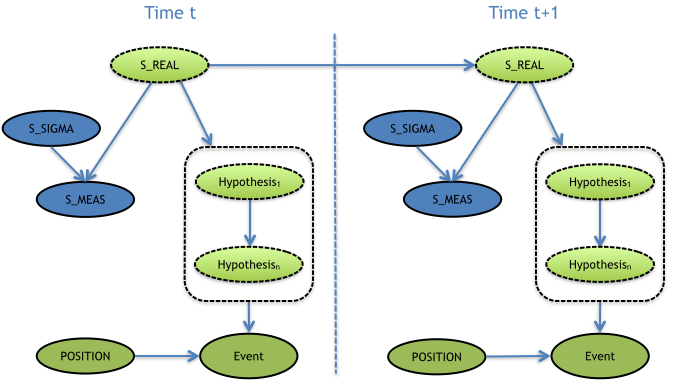
\includegraphics[scale=0.58]{./figures/DaimlerLEdynGeneric}
\end{center}
\caption{\label{Figure:daimlerLEdynGeneric}Daimler dynamic model with several hypothesis.}
\end{figure}



%A DBN induces a number of constraints on the compilation of the network into a computational structure. One constraint relates to transferring the belief state from one time slice to the next where the belief state is the probability distribution over the variables shared by neighbouring time slices. In general, the belief state is transferred as a joint distribution. We have imposed limitations in our dynamic model so that the next state depends only on the current state, and not on the sequence of events that preceded it, i.e. first order Markov model. Although in principle this might seem as a strong limitation, we have reasons to believe that this property might hold in our data. Fig. \ref{Figure:daimlerCorrel} displays, at the top, the sample correlograms for lateral velocity and offset, that is, the correlation of the data with lagged values of themselfves. The partial correlogram (bottom figures) is used to remove the common linear effect of the data in between samples. In our example, for both variables, the correolograms take some time to decay to zero, while the partial correlograms are large for lag one and then small of all other lags. This indicates that the correlation between non consecutive samples is due to the common relationship of these samples and the samples in between \cite{Newton:1988}.

\subsubsection{Earlier prediction of the need for a lane change based on relative dynamics}

Earlier prediction of manoeuvre intentions could be achieved before any development of the trend for lateral evidence has been observed. A first indication of possible lane change intention can be observed through the relative dynamics between one vehicle (EGO or OBJECT) and the vehicles in front of it on the same lane. If a slower vehicle is driving in front of the own vehicle on the same lane, this could be an indication of the need for a lane change. Because to continue its safe driving, the approaching vehicle should either break and reduce its speed to the speed of the vehicle in front or, alternatively, it should change to the neighbour lane, if the neighbour lane is free and no other vehicle is approaching with a higher speed than the own vehicle. A continued safe manoeuvre (of type ``lane follow'' or ``lane change'') is modelled by estimating the TTC (TimeToCollision) to the vehicle in front (on the same lane) or to eventually approaching vehicle (on the neighbour lane). For safe manoeuvre, TTC should be bigger than 1 second, if the own vehicle wants to change to the neighbour lane or if it needs to break to ensure safe driving on the same lane (``lane follow'') . Our assumptions is that this approach will allow us to further increase the prediction horizon for manoeuvre recognition (up to $5$ seconds).

Similarly to the models described in Figure \ref{Figure:daimlerLEdyn},  a new dynamic OOBN is defined with the hypothesis ``relative dynamics'' (REL\_DYN), as shown in Figure \ref{Figure:daimlerreldyn}. Due to confidentiality reasons, we can not give at this stage of the project further details about this model. 

%We can see however that this model have the same general structure that the dynamic models proposed for the previous application scenario. 
% any type of data analysis that supports this hypothesis. 


 

\begin{figure}
\begin{center}
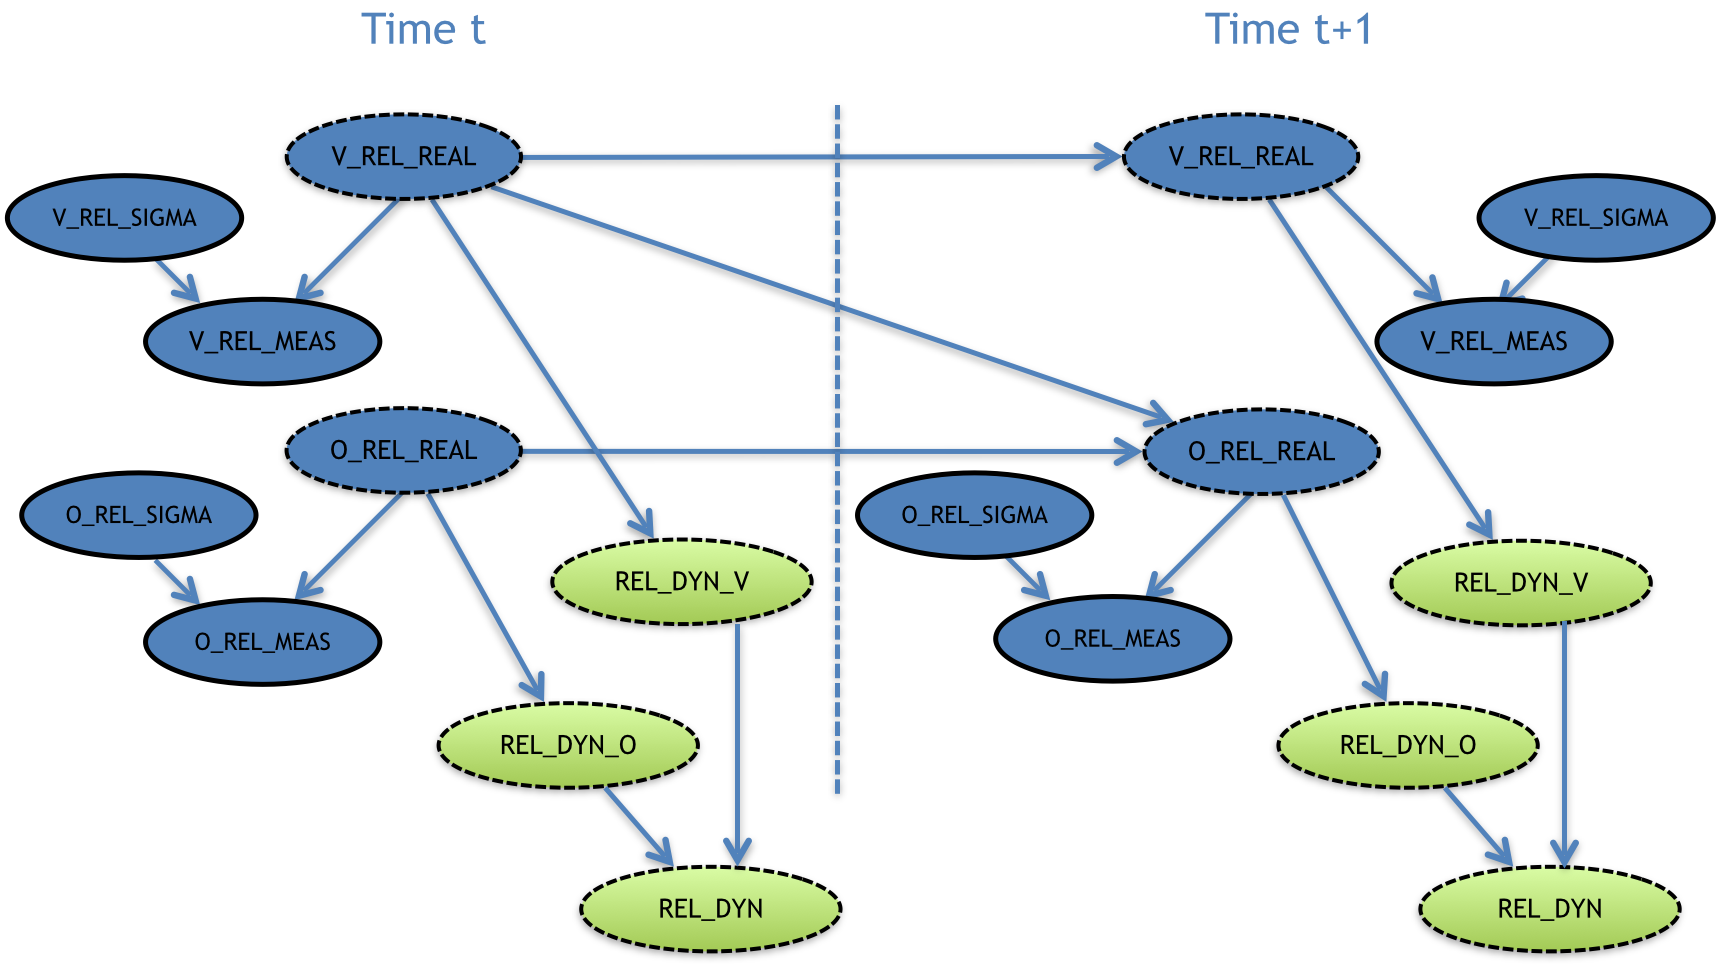
\includegraphics[scale=0.58]{./figures/Daimlerreldyn.png}
\end{center}
\caption{\label{Figure:daimlerreldyn}Daimler Temporal Model with relative dynamics. V\_REAL and O\_REAL refers to the relative velocity and relative distance between the EGO and the car in front, repectively. The other variables with \_MEAS and \_SIGMA suffixes refers to the measured values and the uncertainty of the measurements, respectively, as commented in the previous section for other sensor readings.}
\end{figure}


%This BN fragment  models the hypothesis REL\_DYN with 3 states Left/Follow/RIGHT, utilising the independency assumption for the discrete variables V\_REL\_MEASSURED and X\_REL\_MEASSURED.
%
%If we compare the structure of this network with that of Figure \ref{Figure:daimlerLEdyn}, we can observe two additional nodes:  REL\_DYN\_V\_REL\_OBJ and REL\_DYN\_X\_REL\_OBJ. They are the results of a modelling trick to simplify the EM-learning of parameters from data for the static BN fragment.
%
%\textcolor{red}{Note that the new REL\_DYN hypothesis introduced would require two instances in the OOBN, one for the relative dynamics of the EGO with the OBJ in front, and another one for the OBJ and another OBJ in front of it. Each REL\_DYN would indicate if the EGO and the OBJ cars are going to turn right, left or continue straight.}
%



\subsubsection{Discussion and future models}
The above included proposals are preliminary models designed in line with the expert knowledge facilitated by Daimler. They all try to balance a good level of expressiveness and efficiency during inference.  But, in any case, they should be seen as a first proposal that might be modified/adapted in the future if they do not meet the efficiency and accuracy targets specified in the requirements \cite{Fer14}. 

For application scenario 1 (see Section \ref{Section:Daimler:EarlyRecognition}),  we envision, for example, the possibility of considering not only the temporal dependences between consecutive time steps for the sensor measurements but also, or instead, consider the temporal links between a hypothesis at consecutive time steps (i.e. adding in Figure \ref{Figure:daimlerLEdynGeneric} temporal links between thy hypothesis nodes at different time steps). It seems natural, for instance, that the probability of observing lateral evidence (LE) for the EGO car should be higher given that there was LE at the previous time step. And similarly for the rest of the hypotheses, such as TRAJ or OCCGRID  and the final hypothesis or event that identifies the type of manoeuvre. However adding these type of dependences would greatly increase the complexity of inference in the resulting network because the number of dependencies will be much higher as the DBN is unfolded through the time. As it was described in D1.2 \cite{Fer14}, models in this case are subject to very strong constraints in terms of computational efficiency, so we should be very cautions at this respect. 

Another possible extension that we envision is the consideration of an extra hidden variable to model acceleration for the dynamic model. We believe that assuming that lateral velocity varies according to a constant acceleration can lead to inaccuracies. Figure \ref{Figure:daimlerVel} (a) shows the behaviour of lateral velocity for a given sequence, that in this case corresponds to an EGO-CutIn manoeuvre. At the beginning of the sequence, acceleration is close to constant, but from around time steps 30 to 50 a higher acceleration value should be taken into account. The contour plot on Figure \ref{Figure:daimlerVel} (b) shows a large density of points around lower and higher values of V where the acceleration is constant, but just isolated points in between. Hence, we believe that the dynamic model could benefit from an extra hidden variable to represent acceleration as displayed in Figure \ref{Figure:tempDynAccel}. %(SIGMA and MEAS. variables have been left out for simplicity). 
Thus, the following equation would be considered for velocity at consecutive time steps:

\begin{equation}
V(t) =V(t-1) +A(t-1)dt +\epsilon
\end{equation}

\noindent where $A(t-1)$ denotes the acceleration at time step $t-1$ and $\epsilon$ is again some white noise. In this model, acceleration is assumed to be almost constant between two consecutive time steps: $A(t) = A(t-1) + \epsilon$. 

\begin{figure}
  \centering
  \setlength{\tabcolsep}{0.05pt}
  \renewcommand{\arraystretch}{0.02}
    \begin{tabular}{cc}
    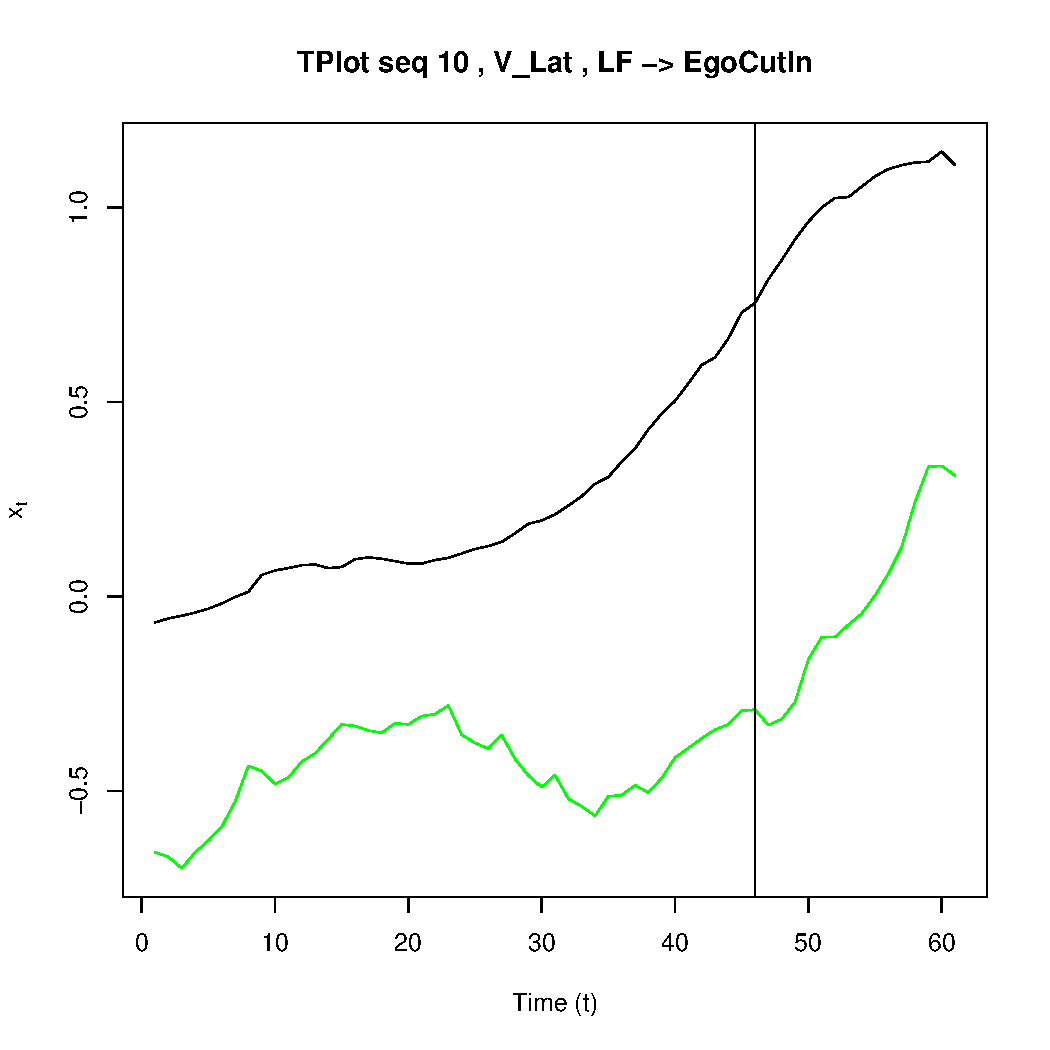
\includegraphics[width=60mm]{figures/DaimlerLE_EGO_L_LE_OBJ_R_EGOCutInVel.pdf}&
    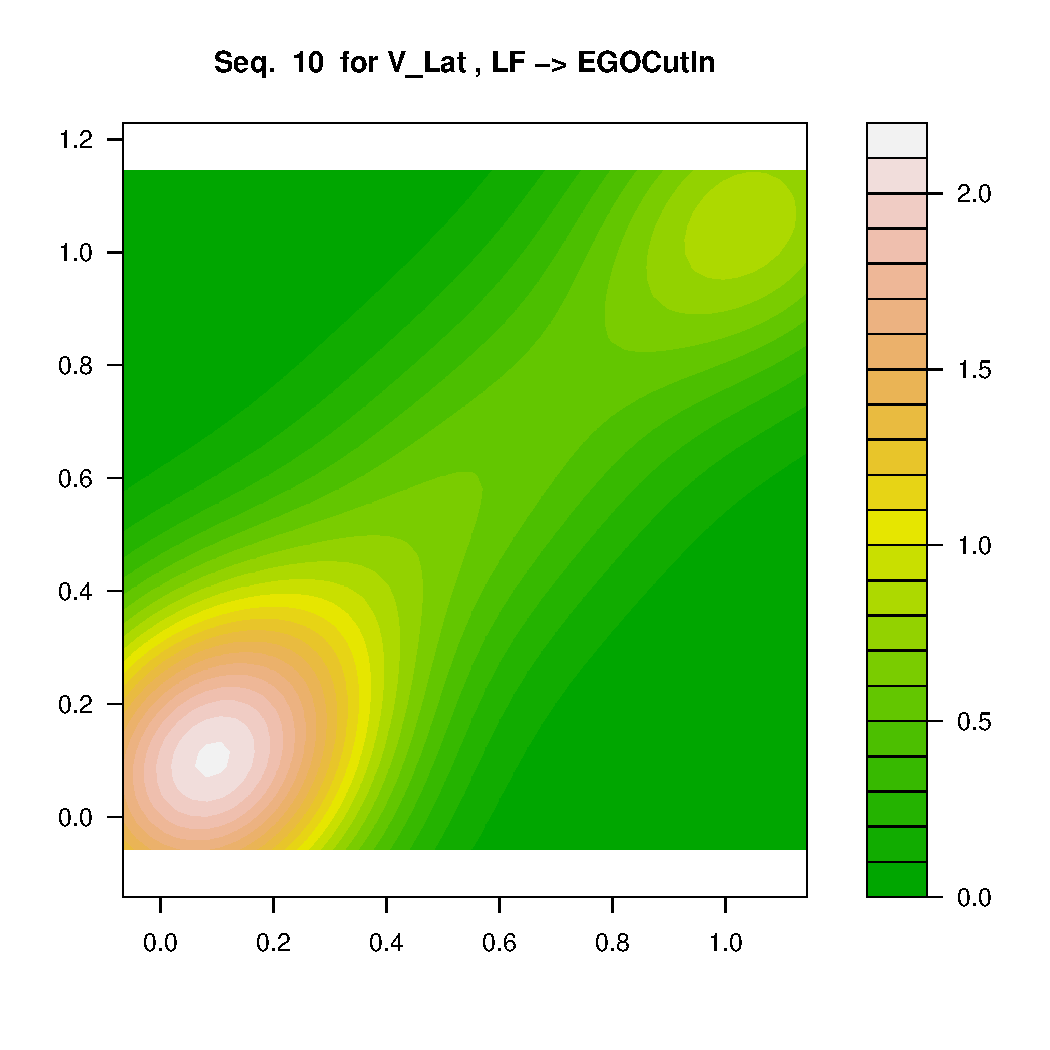
\includegraphics[width=60mm]{figures/DaimlerBivariate_temporal_analysisEGO_LVel.pdf}\\
  \end{tabular}
      \caption{ \label{Figure:daimlerVel}Time and contour plots for $V(t)$ vs $V(t-1)$. Varying acceleration should be considered to capture the variations in the data.}
\end{figure}

\begin{figure}
\begin{center}
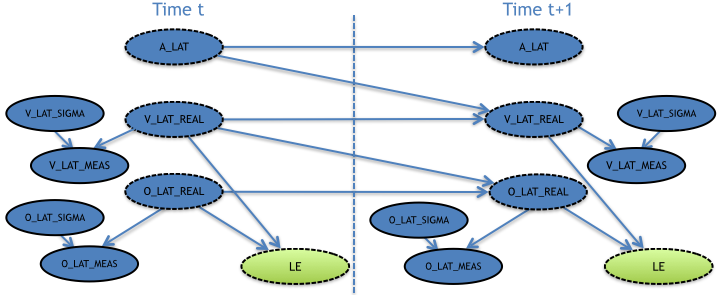
\includegraphics[scale=0.58]{./figures/DaimlertempDynAccel}
\end{center}
\caption{\label{Figure:tempDynAccel}Daimler dynamic fragment for the LE hypothesis with a hidden node for acceleration.}
\end{figure}